\section{Verteilung}
\subsection{Effizienz}
Pareto-Effizienz: Eine wirtschaftspolitische Massnahme ist dann effizient, wenn sie die Situation eines Einzelnen verbessert, ohne andere schlechter zu stellen. 
\subsection{Verteilung}
\begin{itemize}
	\item Die Einkommensverteilung hängt ab von der Produktivität der Arbeitenden.
	\subitem Daher verdienen weniger leistungsfähige Personen weniger.
	\item Will die Gesellschaft dies nicht akzeptieren, so muss umverteilt werden.
	\item Wird zu viel umverteilt, gibt es weniger Anreize zu persönlicher Leistung.
	\item Wird zu wenig umverteilt wird dies als ungerecht empfunden.
	\item Die Herausforderung ist, die Verteilung mit möglichst geringen Anreizen zur Verschwendung von Ressourcen zu erreichen.
\end{itemize}

\subsubsection{Gini-Koeffizient}
\begin{multicols}{2}
Der Gini-Koeffizient sagt nichts über den Wohlstand (Vermögensverteilung) aus, sondern nur über die Einkommensverteilung.\\
Je grösser der Gini-Koeffizient, umso schlechter / unfairer ist die Einkommensverteilung.
\includegraphics[width=\linewidth]{images/gini.jpg}
\columnbreak
\subsection{Umverteilung} 
\textbf{Einkommensquellen}
\begin{itemize}
	\item Lohn
	\item Erträge aus Vermögen
	\item Staatliche Transfers
\end{itemize}
\textbf{Arten der Umverteilung}
\begin{itemize}
	\item Einnahmenseite:
	\begin{itemize}
		\item Progressives Steuersystem (Einkommens- und Vermögenssteuer)
	\end{itemize}
	\item Ausgabenseite
	\begin{itemize}
		\item Direkte Geldtransfers
		\item Verbilligung von staatlichen Leistungen (z.B. Krankenkassenprämien)
	\end{itemize}
\end{itemize}
\end{multicols}

\subsection{Lösungsmöglichkeiten für die Finanzierung der AHV}
Seit 2017 ist die AHV defizitär.\\
Wirtschaftspolitisch direkt beeinflussbare Parameter:
\begin{itemize}
	\item Höhe der Beiträge (MwSt.: unsoziale Steuer, jeder zahlt gleich viel)
	\item Höhe der Renten
	\item Höhe des Rentenalters
\end{itemize}
Wirtschaftspolitisch nur indirekt beeinflussbare Parameter:
\begin{itemize}
	\item Immigration
	\item Geburtenrate
	\item Wirtschaftswachstum (höheres BIP pro Kopf)
\end{itemize}

\clearpage
\pagebreak
\subsection{Umverteilung Ausgabenseite: Sozialwerke}
\centering
\includegraphics[width=0.8\linewidth]{images/sozialwerke.png}
\flushleft
\subsection{Die drei Säulen der Altersvorsorge der Schweiz}
\centering
\includegraphics[width=0.8\linewidth,]{images/dreissaulen.png}
\flushleft

\subsection{BVG}
Bundesgesetz über die berufliche Alters-, Hinterlassenen- und Invalidenvorsorge

\subsubsection{Mindestzinssatz}
\begin{multicols}{2}
Der Mindestzinssatz wird vom Bundesrat festgelegt. Er bietet für die Versicherungsnehmer eine Sicherheit durch eine garantierte Verzinsung des Sparkapitals.\\
Wir werden weniger Pension als heutige Eltern erhalten.
\columnbreak
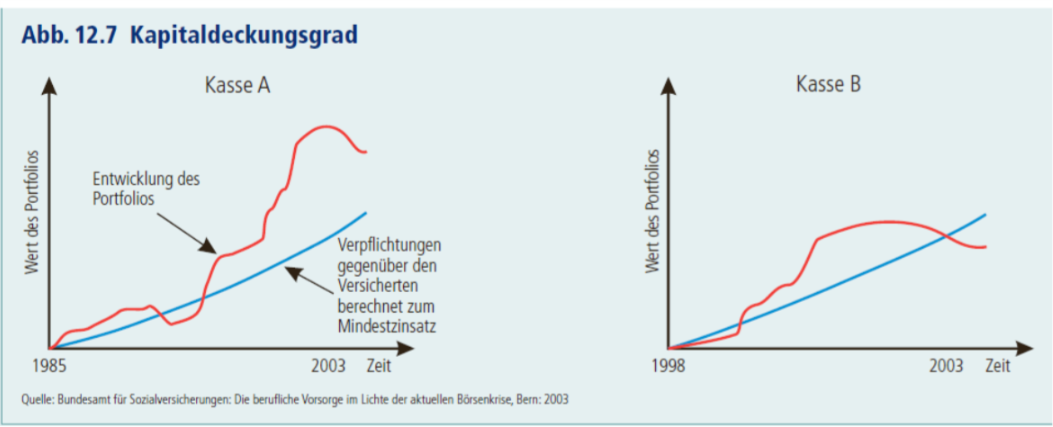
\includegraphics[width=\linewidth]{images/mindestzinssatz.png}
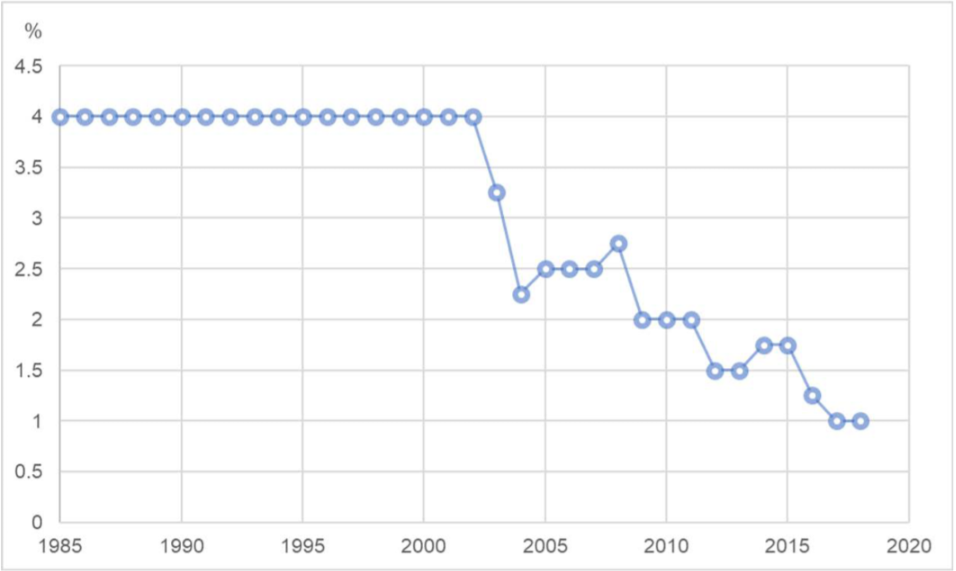
\includegraphics[width=\linewidth]{images/mindestzinssatz2.png}
\end{multicols}

\subsubsection{Umwandlungssatz}
\begin{itemize}
	\item Der Umwandlungssatz legt fest, welcher Prozentsatz des angesparten Vermögens pro Jahr als Rente ausbezahlt werden muss. Dieser wird vom Parlament beschlossen.
	\item Der Umwandlungssatz bedeutet eine Vermögensumverteilung von wenig lang zu länger Lebenden.
	\item 2005 lag der Umwandlungssatz noch bei 7,2\%.
	\item Bis 2014 wurde dieser schrittweise auf den heute gültigen Satz von 6,8\% gesenkt.
	\begin{itemize}
		\item \textasciitilde 15 Jahre bis aufgebraucht $\rightarrow$ tiefer als Lebenserwartung $\rightarrow$ Problem!
	\end{itemize}
	\item Gegen eine vom Parlament geplante Kürzung des Umwandlungssatzes auf 6,4\% wurde 2010 erfolgreich das Referendum ergriffen.
	\item Auch die Senkung des Umwandlungssatzes auf 6,0\% (Abstimmung zur Vorlage "Altersvorsorge 2020") wurde durch das Volk 2017 abgelehnt.
\end{itemize}

\begin{multicols}{2}
\subsection{Armut und materielle Entbehrung}
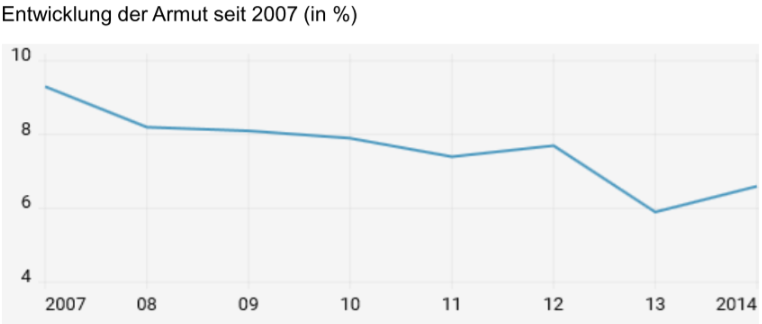
\includegraphics[width=\linewidth]{images/armut.png}
Als \textbf{arm} gelten Personen, die nicht über die finanziellen Mittel verfügen, um die für ein gesellschaftlich integriertes Leben notwendigen Güter und Dienstleistungen zu erwerben. Die Armutsgrenze setzt sich zusammen aus dem Grundbedarf für den Lebensunterhalt, den individuellen Wohnkosten sowie monatlich 100 Franken pro Person ab 16 Jahren im Haushalt für weitere Auslagen.\\
In der EU sind mit 18,6\% der Bevölkerung weitaus mehr Menschen von materiellen Entbehrungen betroffen.\\
Die \textbf{Quote der materiellen Entbehrung} wird beschrieben als finanziell bedingter Mangel in mindestens drei von neun europaweit koordinierten Kategorien:
\begin{itemize}
	\item innerhalb eines Monats unerwartete Ausgaben in der Höhe von 2500Fr. tätigen
	\item eine Woche Ferien pro Jahr weg von zu Hause finanzieren
	\item keine Zahlungsrückstände
	\item jeden zweiten Tag eine fleisch- oder fischhaltige Mahlzeit (oder vegetarische Entsprechung) einnehmen
	\item Wohnung ausreichend heizen
	\item Zugang zu einer Waschmaschine
	\item im Besitz eines Farbfernsehers, eines Telefons und eines Autos sein
\end{itemize}
\end{multicols}

\subsection{Vorschlag zur radikalen Neugestaltung der Sozialwerke (BGE)}
\textbf{Das Bedingungslose Grundeinkommen BGE (Abstimmung 2016)}\\
2012 war der Start der Unterschriftensammlung für ein BGE mit Unterstützung durch Syna, SP, PdA und weitere. Die Volksinitiative ist 2013 erfolgreich zustande gekommen. Sie fordert:
\begin{itemize}
	\item[\-] Art. 100a (neu) bedingungsloses Grundeinkommen
	\item[\-] 1. Der Bund sorgt für die Einführung eines bedingungslosen Einkommens.
	\item[\-] 2. Das Grundeinkommen soll der ganzen Bevölkerung ein menschenwürdiges Dasein und die Teilnahme am öffentlichen Leben ermöglichen.
	\item[\-] 3. Das Gesetz regelt insbesondere die Finanzierung und die Höhe des Grundeinkommens.
\end{itemize}
\textbf{Vorstellungen des Initiativkomitees:}\\
Jede rechtmässig in der Schweiz sich aufhaltende Person erhält ein bedingungsloses Grundeinkommen. Vorgeschlagen wird:
\begin{itemize}
	\item{\makebox[3cm]{Erwachsene\hfill}} 2500.-
	\item{\makebox[3cm]{Kinder\hfill}} 625.-
\end{itemize}
Das Grundeinkommen ersetzt dabei bestehende Einkommen, z.B.:
\begin{itemize}
	\item{\makebox[3cm]{vorher:\hfill}} Lohn 6000.-
	\item{\makebox[3cm]{nachher:\hfill}} Lohn 3500.- und Grundeinkommen 2500.-
\end{itemize}
\textbf{Finanzierung des BGE:}
Der Finanzierungsaufwand des BGE wird vom Initiativkomitee insgesamt mit 209 Mia. (ca. 1/3 des BIP) eingeschätzt.\\
Finanziert soll das BGE (Stand 4.3.2016) wie folgt werden:
\begin{itemize}
	\item{\makebox[3cm]{62 Mia.\hfill}} Durch vollständiges Ersetzen der AHV, Sozialhilfe, Familienzulagen, Stipendien und teilweises Ersetzen von IV, EL, ALV
	\item{\makebox[3cm]{5 Mia.\hfill}} Streichen von Agrarsubventionen sowie Einsparungen bei der "Bürokratie"
	\item{\makebox[3cm]{107 Mia.\hfill}} Verrechnungen des BGE bei den Löhnen (100\% ab 4000.-)
	\item{\makebox[3cm]{34 Mia.\hfill}} Erhöhung der MwSt. um 10\% und höhere Energiesteuern (10 Mia.), "Geschenk" der Pensionskassen (10 Mia.), weitere 14 Mia. noch unklar
\end{itemize}
\clearpage
\pagebreak